\chapter{\IfLanguageName{dutch}{Stand van zaken}{State of the art}}
\label{ch:stand-van-zaken}

% Tip: Begin elk hoofdstuk met een paragraaf inleiding die beschrijft hoe
% dit hoofdstuk past binnen het geheel van de bachelorproef. Geef in het
% bijzonder aan wat de link is met het vorige en volgende hoofdstuk.

% Pas na deze inleidende paragraaf komt de eerste sectiehoofding.

%Dit hoofdstuk bevat je literatuurstudie. De inhoud gaat verder op de inleiding, maar zal het onderwerp van de bachelorproef *diepgaand* uitspitten. De bedoeling is dat de lezer na lezing van dit hoofdstuk helemaal op de hoogte is van de huidige stand van zaken (state-of-the-art) in het onderzoeksdomein. Iemand die niet vertrouwd is met het onderwerp, weet nu voldoende om de rest van het verhaal te kunnen volgen, zonder dat die er nog andere informatie moet over opzoeken \autocite{Pollefliet2011}.
\section{Secrets Management}
\label{sec:secrets management}
Om te verstaan wat \textbf{secrets management} inhoudt, worden de termen \textbf{secrets} en \textbf{secrets sprawl} weer verduidelijkt. Secrets impliceert een verzameling van gevoelige gegevens. Deze dienen als sleutel om digitale authenticatie uit te voeren, om toegang te krijgen tot een systeem \autocite{Dadgar2018}. Enkele voorbeelden zijn:

\begin{itemize}
    \item Gebruikersnaam en wachtwoord
    \item API tokens
    \item SSH keys
    \item Database inloggegevens
\end{itemize}

Deze gegevens zullen een secret sprawl veroorzaken wanneer deze niet onderhouden worden op de juiste manier. Secret sprawls ontstaan wanneer sensitieve gegevens, in allerlei plaatsen gebruikt worden om mee te werken. Bijvoorbeeld in automatisatie processen (Ansible, Puppet, Chef), containerized applications (Kubernetes, Red Hat OpenShift, Docker), Continuous Integration/Continuous Deployment (CI/CD) (TeamCity, Jenkins). Vroeg of laat belanden bestanden met onbewerkte tekst van gevoelige data in versiebeheer systemen, applicatie systemen of worden deze als lokale variabele gebruikt. Veel problemen ontstaan wanneer een bedrijf veel te laat beseft dat ze met een secret sprawl zitten, maar één van de grootste problemen is dat het bedrijf in meerdere locaties gevoelige gegevens heeft staan en dat er geen duidelijk overzicht is van waar deze gegevens zitten. Het bedrijf zal dan ook niet weten welke personen toegang hebben om deze gegevens te bekijken \autocite{Tozzi2020} \autocite{Dadgar2018}. 
\newline 


Secrets management streeft naar een situatie waar secret sprawls vermeden worden, de gegevens geëncrypteerd zijn, dat de distributie van deze gegevens beheerd worden vanuit een gecentraliseerde locatie en als laatste dat deze gegevens gebruikt kunnen worden bij automatische processen zonder enige manuele tussenkomst. \textcite{Somerfield2015} legde uit hoe de uitdagingen die deze problemen stelden, werden aangegaan. Hier wordt het \textit{Orchestrator Decryption} model uitgelegd \autocite{Somerfield2015}. 

\subsection{Orchestrator Decryption} 

\begin{figure}[htbp]
\centerline{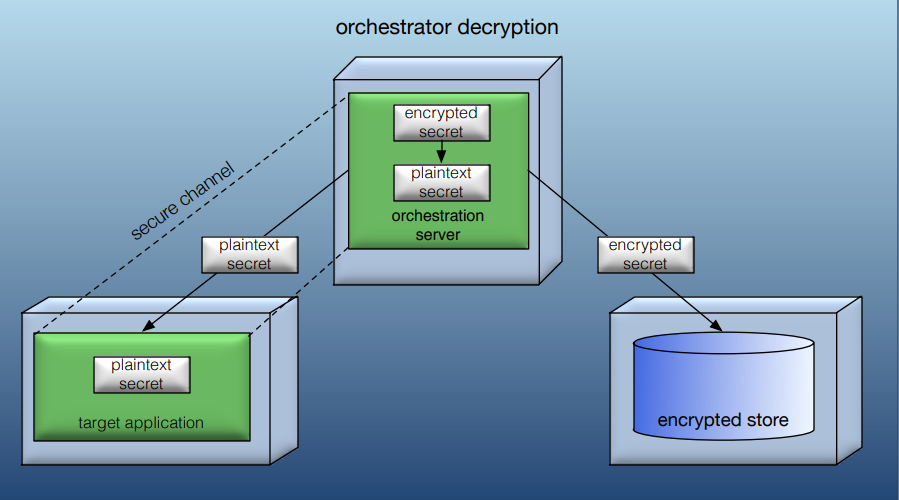
\includegraphics[width=400]{bachproef/img/orchestrator decryption.png}}
\caption{Orchestrator Decryption \autocite{Somerfield2015}}
\label{fig}
\end{figure}

Bij \textbf{orchestrator decryption} kijken we vooral naar \textit{configuration management tools} zoals ansible, chef, puppet. Deze applicaties kunnen met een tussenkomst van bijkomende applicaties gevoelige data veilig houden wanneer deze niet gebruikt worden, deze zijn in rust geëncrypteerd. Wanneer de geëncrypteerde secret wordt opgeroepen bij een opdracht wordt deze door de orchestration tool naar een \textit{plaint text} secret gedecrypteerd, met andere woorden wordt deze omgevormd tot onbewerkte tekst. Een voorbeeld van een orchestration georiënteerde tool is ansible. Deze tool kan gebruik maken van ansible vault om een vorm van secret management aan te gaan maar wordt gelimiteerd door een aantal factoren waardoor het binnen het model van \textit{Orchestrator decryption} blijft \autocite{Somerfield2015}. Om dit duidelijk uit te leggen, wordt in het algemeen uitgelegd wat ansible is en waarvoor deze tool gebruikt wordt. Verder wordt er ook uitgelegd hoe ansible vault hierop inspeelt. \newpage

\subsection{Ansible}  
\label{ch:ansible}

Ansible\footnote{\href{https://www.ansible.com}{Ansible website}} is een open-source, configuration management tool (CMT) die door Red Hat\footnote{\href{https://www.redhat.com}{Red Hat website}} onderhouden wordt sinds 2015. Ansible is tegenwoordig op de voorgrond als het om geautomatiseerd configuratie, coördinatie en beheer van computer systemen gaat. Tegenwoordig is ansible de meest gebruikte CMT waar het applicaties zoals Chef, Salt en Puppet overtreft \autocite{Rayome2019}. Het is ook handig voor simpele gebruikers die alledaagse taken willen uitvoeren binnen simpele netwerken, en niet alleen op één computer. Deze tool geeft je de mogelijkheid om binnen een complex netwerk van computers, vanuit één centraal punt, configuraties te deployen en systemen te beheren. Dit lost problemen op zoals bijvoorbeeld, wanneer men op verschillende computers het zelfde doel wilt bereiken zonder deze taak manueel opnieuw en opnieuw te doen op elke computer. Men kan via een centrale computer opdrachten versturen naar één of meerdere locaties tegelijkertijd. Hierdoor wordt ook het concept van menselijke fout vermeden.

In Ansible wordt er een onderscheid gemaakt tussen de control node en de managed node. De control node is een computer die ansible draait waar alle taken uit verzend worden. Deze taken voeren wijzigingen uit op de managed nodes. Ansible's manier van werken is allereerst een verbinding vast te leggen met de managed nodes, daarna wordt tijdelijk een programma gepushed dat uitgevoerd wordt tijdens deze verbinding. Deze programma’s noemen ansible modules. Bij het einde van een taak wordt de module lokaal op de node verwijderd en sluit ansible de verbinding met de node. Ansible is \textit{agentless} gebaseerd. Dit wilt zeggen dat op de managed nodes geen ansible applicatie aanwezig moet zijn die de configuraties verkrijgt en verwerkt. Ansible maakt gebruik van \textit{connection plugins} waaruit \textbf{SSH} (Secure Shell) de meest gebruikte is. Deze worden gebruikt om een verbinding vast te leggen met linux / unix hosts. Voor Windows hosts wordt \textbf{WinRM} (Windows Remote Management) gebruikt \autocite{RedHatAnsible2021}. 

\begin{figure}[htbp]
\centerline{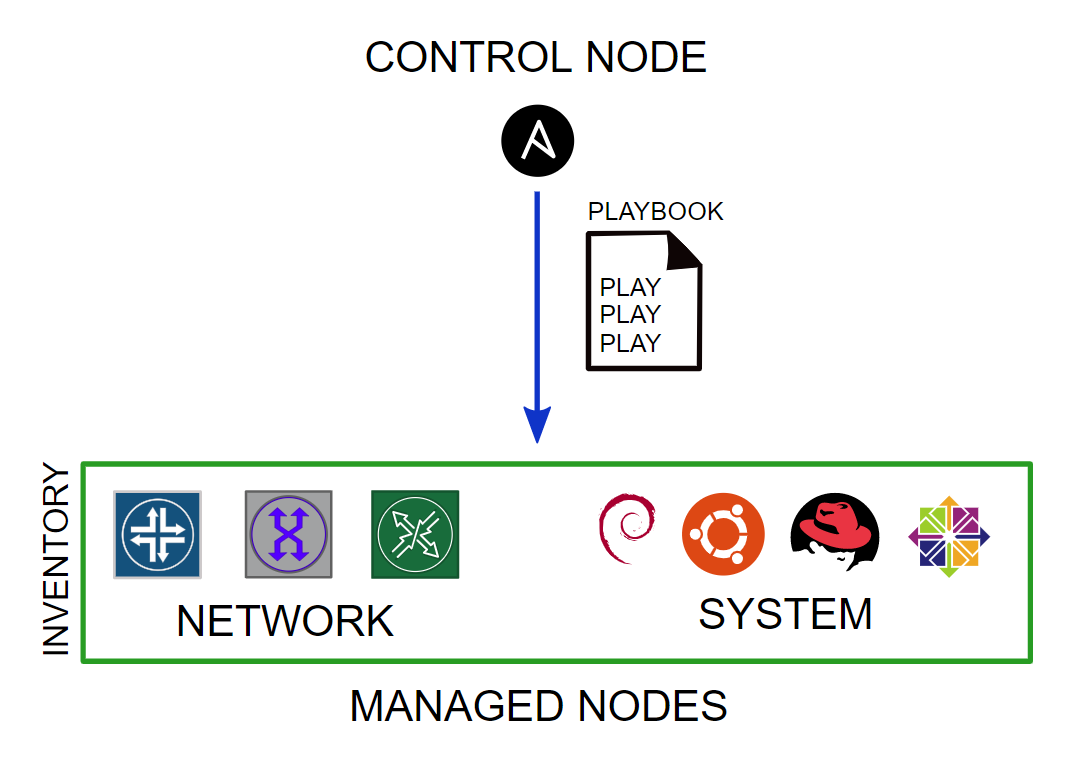
\includegraphics[width=250]{bachproef/img/AnsibleArchitecture.png}}
\caption{Werking ansible met control en managed nodes \autocite{Coding2019}}
\label{fig}
\end{figure}
\newpage
Omdat Ansible een tool omtrent automatisatie is, heeft deze tool dan ook instructies nodig. De instructies die ansible uitvoert zijn idempotent. Dit wilt zeggen wanneer bij een instructie een opdracht wordt uitgevoerd, maar er valt niets te wijzigingen in het systeem, zal ansible hier niets doen. Ansible zal deze stap overslaan en de volgende opdracht proberen uitvoeren \autocite{Coding2019}. Deze instructies worden als taken opgenomen in een \textbf{YAML} (Yet another Markup Language) bestand \autocite{ingerson80yet}. Een jaar na de introductie van het YAML formaat is de betekenis van het acroniem verandert naar (YAML Ain't Markup Language) \autocite{VugtYAML}, dat is inderdaad een recursief acroniem. %Hieronder wordt er een voorbeeld gegeven van een inventory file en een playbook. De \textit{inventory file} kan een generiek bestand zijn zonder extensie, een ansible playbook is altijd in een YAML bestandsformaat. 


\begin{figure}[hbtp]
    \caption{Voorbeeld inventory file ansible}
    %\label{code.1}
    \begin{lstlisting}[language=yaml,frame=single]
        [web]
        be-dev-ansible-01
        be-dev-ansible-02
        
        [web:vars]
        ansible_python_interpreter=/usr/bin/python3
        ansible_ssh_user=John 
        ansible_ssh_pass=JohnSecure123
    \end{lstlisting}
    \label{fig:inventorypass}
\end{figure}
De inventaris afgebeeld op figuur \ref{fig:inventorypass}, impliceert dat de machines, \textit{be-dev-ansible-01} en \textit{be-dev-ansible-02}, met de extra variabelen opgeroepen kunnen worden als groep web. Hierdoor gebruiken playbooks volgende python versie, volgende SSH gebruikersnaam en het bijbehorende wachtwoord bij het uitvoeren van volgende taken.


\begin{figure}[hbtp]
    \caption{Voorbeeld ansible playbook}
    %\label{code.1}
    \begin{lstlisting}[language=yaml,frame=single]
    1.	---
    2.	- hosts: web
    3.	  tasks:
    4.      - name: permit traffic on port 10000-10001/tcp
    5.          firewalld:
    6.          port: 10000-10001/tcp
    7.          permanent: yes
    8.          state: enabled
    9.	    - name: ensure nginx is at the latest version
    10.	      apt: name=nginx state=latest
    11.	    - name: start nginx
    12.	      service:
    13.	          name: nginx
    14.	          state: started
    \end{lstlisting}
    \label{fig:playbookvb}
\end{figure}

In figuur \ref{fig:playbookvb} wordt er geïllustreerd hoe ansible voor de groep web, volgende taken gaat uitvoeren. Allereerst wordt er gezien of de TCP poorten 10000 en 10001 open staan, indien dit het geval is gebeurt er hier niets en gaat het playbook verder. Dit wordt aangeduid door het \textit{state: enabled} gedeelte. Verder wordt er gekeken om nginx te installeren via de \textit{command-line utility commando} apt, als nginx reeds geïnstalleerd is zal er gekeken worden of die van de laatste versie is. Na het uitvoeren of het overslaan van deze taak wordt er voor gezorgd dat nginx gestart is als dit niet het geval is. Moest er bijvoorbeeld iets intern mis gaan bij een van de taken, zal deze in het output scherm als een \textit{fatal error} verschijnen met een boodschap waarom dit gebeurt is en voor welke host.

In het vorige voorbeeld werd er aangetoond hoe problematisch het is wanneer \textbf{secrets} in een productieomgeving in allerlei bestanden als onbewerkte tekst terechtkomen. Wanneer er meerdere playbooks worden aangemaakt die elk gevoelige data bevatten om de automatisatie te behouden. Is het onvermijdelijk dat deze vroeg of laat op source control terechtkomen. Eens dat gebeurt, is het al te laat. Via audit kan men vorige versies bekijken van \textit{commits} en gevoelige data in de vorm van onbewerkte tekst zien \autocite{Wehner2015}. Iedereen die in deze \textit{public} of \textit{private repository} zit kan de secrets zo bekijken, en men weet niet wie deze gegevens reeds bekeken heeft. 

\subsection{Ansible Vault} 

In het geval van ansible en playbooks biedt ansible vault een mogelijke oplossing, Ansible Vault\footnote{\href{https://docs.ansible.com/ansible/2.9/user\_guide/vault.html}{Ansible Vault website}} is een tool voor ansible dat bestanden met gevoelige data encrypteert. Dit biedt de mogelijkheid aan zodat alle taken kunnen uitgevoerd worden tijdens ansible taken die gegevens gebruiken die niet zichtbaar mogen zijn. Ansible zal de bestanden automatisch decrypteren tijdens looptijd, mits de sleutel voorzien is. Via één of meerdere wachtwoorden kan men inhoud encrypteren en decrypteren \autocite{RedhatAnsibleVault}. Dit lost het probleem op dat gegevens niet meer zichtbaar zijn voor de buitenwereld. Maar ansible vault lost jammer genoeg het probleem niet volledig op. Wanneer ansible modules verstuurt worden naar een managed node, worden deze tijdelijk opgeslagen in een verborgen directory. Hier staan deze gegevens zonder encryptie. Dit wilt zeggen dat de gebruikte data, bijvoorbeeld wachtwoorden, overgezet worden op het bestandssysteem van de remote host. Zoals eerder verteld kan ansible alternatieve connection plugins gebruiken om een verbinding met een remote host vast te leggen. Als men SSH gebruikt zal de data geëncrypteerd en veilig zijn tijdens het versturen van de modules. Dit beveiligt de data tegen potentiële \textbf{sniffing attacks}. Dit is een tactiek die gebruikt wordt om data te achterhalen tijdens netwerk connectiviteit. Zo kunnen gegevens in onbewerkte tekst achterhaald worden \autocite{Passi2018}. Eens data verzonden is, kan het zijn dat deze toch op de remote host geschreven worden zonder enige encryptie. Dit kan bijvoorbeeld gebeuren wanneer de omgevingsvariabele \textbf{ansible\_keep\_remote\_files} gebruikt wordt. Hiermee blijven gebruikte modules op de remote host staan. Moest deze omgevingsvariabele niet gebruikt worden kan het nog altijd zijn wanneer een verlies van connectiviteit zich plaatsvindt, de modules op de remote host niet verwijderd zijn. Deze blijven daar tot ze manueel verwijderd worden \autocite{GB2018}. Verder is er ook nog de mogelijkheid om de omgevingsvariabele \textbf{no\_log} te gebruiken en deze op \textit{true} te stellen. Dit zorgt er voor dat wanneer de modules weergeven worden in het systeem log, de gevoelige data verborgen blijft. Dit wordt afgebeeld op figuur \ref{fig:nolog} \autocite{GB2018}.
\newpage

Zoals bij ansible vault getoond werd, is het een last om er voor te zorgen dat secrets niet gelekt worden bij het uitvoeren van taken en bij het beheren van bestanden met deze data. Het kanaal waarmee secrets verstuurd worden is niet altijd veilig genoeg om op te vertrouwen. Het beheer van alle secrets via de ansible vault manier is dan ook niet efficiënt in een ondernemingsomgeving. Er is geen vorm van rotatie zodat gegevens na zoveel tijd aangepast worden. Als een persoon een wachtwoord vergeet voor een bestand geëncrypteerd door ansible vault zijn die gegevens zo goed als verloren. De nadelen zijn hier veel te groot en het grootste probleem bij secrets management van secrets centraal te beheren is hier niet opgelost. 

\begin{figure}[htbp]
\centerline{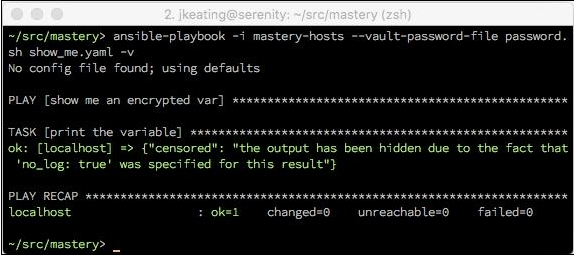
\includegraphics[width=300]{bachproef/img/nolog.png}}
\caption{gebruik van 'no\_log: true' in ansible \autocite{GB2018}}
\label{fig:nolog}
\end{figure}

\newpage
\subsection{Application-Pull}

\begin{figure}[htbp]
\centerline{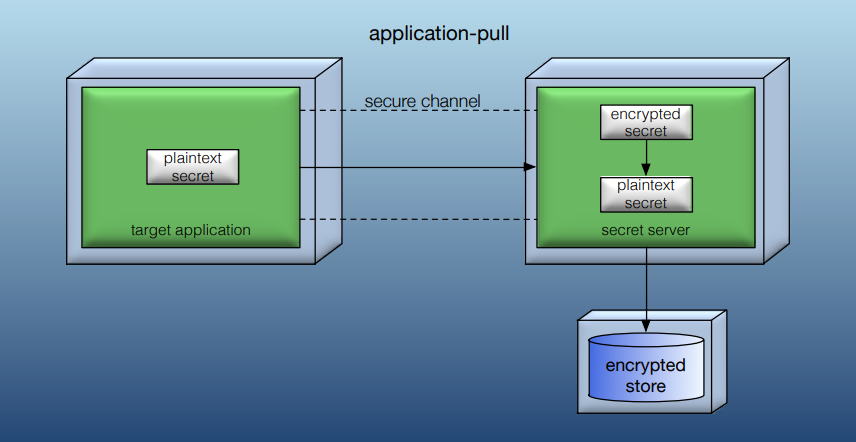
\includegraphics[width=400]{bachproef/img/application-pull.png}}
\caption{Application-pull \autocite{Somerfield2015}}
\label{fig}
\end{figure}

Een model dat meer aansluit bij het principe van secrets management is \textbf{application-pull}. Hierbij kan een persoon, of een service, zich via een systeem laten authenticeren om toegang te krijgen tot een locatie waar secrets beheerd worden. Via een beleid wordt er bepaald of toegang verleend wordt. Alles gebeurt nu ook vanuit een gecentraliseerd punt. Dit is een verbetering en een stevig concept dat meer aansluit bij secret management. Deze applicaties garanderen een aantal sterke punten, namelijk:

\begin{itemize}
    \item \textit{Central management}
    \item \textit{Access policies}
    \item \textit{Auditing}
    \item \textit{Ephemeral credentials}
    \item \textit{Compartmentalization}
    \item \textit{Facilitates rotation}
\end{itemize}

Dit zijn belangrijke kenmerken voor een secrets management systeem. Vault van Hashicorp is één van de applicaties die \textit{application-pull} duidelijk verwoordt. Volgens \textcite{Somerfield2015} was dit in 2015 een applicatie die al in de juiste richting ging \autocite{Somerfield2015}. We zijn ondertussen, bij het schrijven van deze thesis, zes jaar verder.  
%Hier zijn een aantal \textbf{secret management platform} die vandaag de dag het dichtst zijn om \textbf{secrets} de baas te zijn waar ook over besproken zal worden \autocite{Morris2020}:
\newpage

\subsection{Hashicorp Vault}
\label{sec:Hashicorp vault}

Hashicorp, Inc.\footnote{\href{www.hashicorp.com}{Hashicorp website}} is een softwarebedrijf opgericht door Mitchell Hashimoto en Armon Dadgar in 2012. Ze bieden open-source tools en commerciële producten aan die ontwikkelaars de mogelijkheid aanbiedt om applicaties op te zetten in een multi-cloud omgeving. Hashicorp staat bekend voor Vagrant en Terraform. Maar nu gaat de focus naar Vault. Vault is een \textbf{secret management tool} die ontworpen is om gecentraliseerd gevoelige gegevens te bewaren en toegang te beheren tot deze data in een omgeving met weinig vertrouwen. Het kan gebruikt worden om gevoelige data op te slaan en om dynamisch toegang te genereren voor andere applicaties en services \autocite{Lugger2020}. Hashicorp is al jaren mee om een oplossing te zoeken tot de probleemstelling die gemaakt werd door \textbf{secrets} te beheren via een optimale manier. Via vault hopen zij het grootste deel van deze problemen aan te gaan via drie niveau 's \autocite{Dadgar2018}.

\subsubsection{Niveau 1: Central Management}
In het eerste niveau wilt vault het \textbf{secrets sprawl} probleem tegengaan, hiermee worden alle \textbf{secrets} in een centraal punt verzameld. Deze gegevens worden gedecrypteerd en zo behouden gedurende de drie stadia van data, namelijk: \textit{at rest}, \textit{in transit}, en \textit{in use}. Gegevens belanden niet meer in source control of dergelijke zaken, en staan veilig en gedecrypteerd in één locatie. Een volgend punt is de toegangscontrole die vergemakkelijkt wordt. In tegenstelling tot een bitbucket repository van een bedrijf waar iedereen toegang tot heeft, kan men beheren welke gegevens gezien en gebruikt kunnen worden door welke applicaties, alsook welke personen. Daarnaast is er ook een \textit{audit trail} die gebruikt kan worden om na te gaan welke gegevens gebruikt zijn geweest door applicaties en personen \autocite{Dadgar2018}.

\subsubsection{Niveau 2: Dynamic Secret}

Bij dit volgende niveau wordt de probleemstelling benaderd waarbij niet alle applicaties juist omgaan met secrets. Men kan optimaal het eerste niveau beheren maar toch secrets laten lekken door applicaties die deze gegevens gaan gebruiken. Applicaties kunnen bijvoorbeeld secrets loggen naar een log systeem, ze kunnen in diagnostische rapporten verschijnen of zelf opgenomen worden door monitor applicaties als deze actief zijn. Hieruit kan een besluit genomen worden dat applicaties een slechte werking kunnen hebben met secrets. Om dit probleem op te lossen maakt vault gebruik van \textit{ephemeral credentials}. Dit zijn vluchtige gegevens die dynamisch aangemaakt kunnen worden. Met andere woorden zullen deze gegevens na een bepaalde duur niet meer geldig zijn. Een volgende stap is dat men deze gegevens gaat compartimentaliseren om duidelijker de bron van schade terug te vinden. Als voorbeeld heeft men 40 web servers die allemaal dezelfde gegevens gebruiken om een connectiviteit vast te leggen met een databank, een \textbf{shared secret}. Eens deze gegevens gelekt worden kan men moeilijk weten van waar deze gegevens gelekt zijn geweest. Als men voor elke web server unieke gegevens gebruikt, zal men weten dat er bijvoorbeeld een lek heeft plaatsgevonden bij webserver zeven. Hiermee kan men dan ook de gegevens die webserver zeven gebruikt intrekken en deze isoleren van de andere webservers. Indien alle webservers dezelfde gegevens zouden gebruikt hebben, zouden al deze webservers onderbroken worden. Met andere woorden \textit{dynamic secrets} gaan boven \textit{shared secrets} \autocite{Dadgar2018}.

\subsubsection{Niveau 3: Encrypt as a Service}

Het laatste niveau dat wordt aangekaart is hoe externe applicaties die gebruik maken van vault, data verkrijgen, en deze data juist gebruiken wanneer deze \textit{at rest} zijn. Men kan bijvoorbeeld kijken naar de situatie wanneer encryptie sleutels beheerd worden in vault. Deze sleutels worden aan applicaties verleend om cryptografie toe te passen op de data. Applicaties implementeren cryptografie vaak niet op een juiste manier, dit is ook iets dat \textcite{duong2011cryptography}
%Thai Duong en Juliano Rizzo 
hebben aangekaart in een onderzoek waar ze aantonen hoe cryptografie misbruikt wordt in de security designs van een groot deel van het web. Hun focus ging naar ASP.NET. Vault heeft dit probleem waargenomen en stelde zich de vraag hoe ze het voorkomen om een verzameling van encryptie sleutels te beheren en deze te verlenen aan applicaties waar zij cryptografie uitvoeren. Dit is een concept dat is uitgegroeid tot een hele service genaamd \textit{Encrypt as a Service}. Hier geeft vault de mogelijkheid om \textit{named keys} aan te maken. Dit kunnen bank gegevens zijn, krediet kaart gegevens, een identificatienummer, ... Hier worden \textit{High level API's} gebruikt om transactie 's uit te voeren met deze gegevens zoals encrypteer, verifieer, teken. Bij applicaties waar zulke transacties gebeuren, wordt vault via een API aangeroepen om deze zorgvuldig uit te voeren, zonder de nood van de \textit{named keys} en hun gegevens te delen met de applicatie. De implementatie voor dit proces wordt behandeld door vault, men moet applicaties niet vertrouwen om \textit{high level operations} zorgvuldig uit te voeren, en de key management gebeurt ook nog altijd door vault. Deze worden afgeschermd bij de andere applicaties \autocite{Dadgar2018}. 

Via vault werd er aangetoond hoe secrets management een vooruitgang heeft gehad voor secrets te beheren. Door de opkomst van cloud computing zijn er ook een tal secrets management systemen ontstaan in de vorm van cloud oplossingen. Azure Key Vault is een voorbeeld, van Microsoft Azure. Maar eerst wordt in het algemeen uitgelegd wat cloud computing is en de basis hier omtrent.
\newpage


\section{Cloud Computing}
\label{sec:cloud oplossingen}

Volgens de \textbf{\textit{national institute of standards and technology}}\footnote{\href{https://www.nist.gov/}{Nist website}} is cloud-computing (CC) een model, waar services aangeboden worden via een netwerk toegang (internetverbinding) naar een gedeelde netwerkpool van configureerbare ICT-middelen. Deze zijn makkelijk en snel lanceerbaar met het minimum aan moeite zonder enige tussenkomst met de service provider \autocite{mell2011nist}. Dit impliceert dat applicaties, services en data door een eindgebruiker gebruikt kunnen worden via een gebruikersinterface \autocite{malathi2011cloud}. Een heel simpel voorbeeld is het gebruik van e-mail services, zoals: Outlook, Gmail, ... Bij deze zaken heb je juist een computer met een internet verbinding nodig. Dan kan je gebruik maken van de e-mail services die worden aangeboden door een externe provider. Verder duidt het \textit{national institute of standards and technology} aan dat het CC model opgebouwd is uit vijf essentiele karakteristieken, namelijk:

\begin{itemize}
    \item On-demand self service
    \item Broad network access
    \item Measured service
    \item Resource pooling
    \item Rapid elasticity
\end{itemize}

Bij \textbf{\textit{on-demand self service}} zullen de gebruikers met de gegeven resources automatisch kunnen werken zonder tussenkomst van de service provider. Verder zorgt \textbf{\textit{broad network access}} ervoor dat de aangeboden services toegankelijk zijn via een netwerkverbinding. \textbf{\textit{Measured Service}} volgt het principe dat de gebruiker betaalt voor wat men gebruikt, zo is er geen verspilling van resources. Dit wordt ook wel eens het \textbf{\textit{pay as you go}} model genoemd. \textbf{\textit{Resource Pooling}} volgt het principe dat service providers computing resources aan meerdere consumenten aanbieden met de noden van de klant voor het gebruik van virtuele en fysieke middelen. Het geeft een meerwaarde dat gebruikers de zelfde apparatuur gebruiken voor zowel gebruiker als provider. Als laatste is \textbf{\textit{Rapid elasticity}} de eigenschap dat een service \textit{elastisch} moet zijn wat impliceert dat een service moet kunnen op- en afschalen om aan de gegeven capaciteit te voldoen. Met andere woorden is het belangrijk dat er bij piekbelasting moet kunnen worden opgeschaald zonder enige moeite om voor geen storingen te zorgen, verder bij rustige perioden moet er dan ook weer kunnen worden afgeschaald. In kort zijn dit de vijf hoofd kenmerken van cloud computing. Het model is ook nog opgebouwd uit drie \textbf{service models} en vier \textbf{deployment models} die later in deze thesis aan bod komen \autocite{mell2011nist}.
\newpage

Tegenwoordig kent de wereld een aantal grote spelers bij het aanbieden van cloud oplossingen waaronder:

\begin{itemize}
    \item Amazon Web Services (AWS) \footnote{\href{https://aws.amazon.com/}{Amazon AWS website}}
    \item Microsoft Azure \footnote{\href{https://azure.microsoft.com/nl-nl/}{Microsoft Azure website}}
    \item Google Cloud \footnote{\href{https://cloud.google.com/}{Google Cloud website}}
    \item Alibaba Cloud \footnote{\href{https://eu.alibabacloud.com/en}{Alibaba Cloud website}}
    \item Digital Ocean \footnote{\href{https://www.digitalocean.com/}{Digital Ocean website}}
\end{itemize}

 Dit zijn voorbeelden van cloud providers die een public cloud omgeving aanbieden. Hier betaalt de gebruiker voor het gebruik van de ter beschikking gestelde resources. Cloud providers zoals AWS en Microsoft Azure hanteren het eerder besproken concept van \textbf{\textit{Measured Service}} zelfs. Ze bieden hun services aan volgens een \textbf{\textit{Pay as you go}} subscriptie model zodat men betaalt voor wat men uiteindelijk gebruikt. Zo worden bijvoorbeeld bedrijven niet aangerekend voor resources die ze niet gebruiken op het moment zelf. maar ze hebben wel de toegang om deze te gebruiken. Dit is handig wanneer bijvoorbeeld doorheen de dag veel gebruik gemaakt wordt van bepaalde resources maar tijdens de nacht de curve daalt. Verder proberen cloud providers de \textbf{\textit{Quality of Service}} optimaal te houden tegenover de eindgebruiker in een dynamische omgeving. Door de voortdurende groei en optimalisatie van cloud computing komen telkens nieuwe mogelijkheden aan bod voor ontwikkeling van applicaties en systemen \autocite{mell2011nist}. CC zorgt er uiteindelijk voor dat bedrijven kunnen opereren zonder een ouderwetse infrastructuur. Natuurlijk zijn er mogelijkheden waarmee er gecombineerd kan worden met reeds bestaande infrastructuur. Hierdoor noemt het ook cloud \textbf{oplossingen}, voor elk probleem en elke situatie is er wel een oplossing.
\newpage

\subsection{Deployment Models}
\label{sec:Deployment models}

\subsubsection{Public cloud}

\begin{figure}[htbp]
\centerline{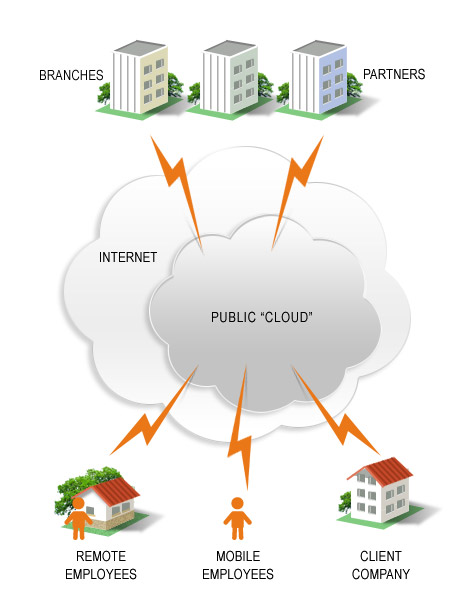
\includegraphics[width=250]{publicCloud.jpg}}
\caption{\textit{public cloud figuur \autocite{mizitechinfo}}}
\label{fig}
\end{figure}

Eerder werd er gesproken over een aantal cloud providers. Deze bieden namelijk diensten aan, die als eerder vermeld een \textbf{\textit{Pay as you go}} gebaseerde subscriptie volgen. Gebruikers betalen bijvoorbeeld voor de \textbf{CPU cycles}, of met andere woorden het gebruik van processor krachten, gebruikte opslag of de gebruikte bandbreedte. Het grootste voordeel hiervan is dat bedrijven zich geen zorgen moeten maken om uitbreidingskosten of het beheren van deze infrastructuur. Er moet niet worden gekeken om een locatie te voorzien, om deze machines te laten draaien want dit wordt al gedaan voor de eindgebruiker. Indien er toch wordt uitgebreid voor meer rekenkrachten of als dit juist verminderd wordt, is dit maar binnen enkele muisklikken te doen \autocite{Sullivan2015PAYG}. Takken zoals beveiliging wordt door de cloud provider optimaal verzorgd. Dit is natuurlijk ook een risico dat gebruikers en bedrijven op zich nemen omdat hun gegevens door een externe partij beheerd wordt. Voor veel bedrijven is dit een serieuze afknapper samen met het feit dat de resources gedeeld worden met andere gebruikers \autocite{cbtnuggets_2019}. Wanneer een bepaalde cloud provider het slachtoffer wordt van een gegevens lek, is de kans natuurlijk groot dat de gegevens van de gebruikers gelekt worden. Dit is geen prettige scenario wanneer gevoelige data geëncrypteerd zou moeten zijn. Door gebruik te maken van een public cloud is dit iets wat bedrijven niet altijd onder controle hebben voor wanneer dit evenement plaats vindt. Door het gebruik van andere \textbf{deployment models} kan dit wel nog tegengewerkt worden.


\subsubsection{Private Cloud}

In tegenstelling tot public cloud waar bedrijven hun data niet volledig in eigen beheer hebben, is dit bij private cloud wel het geval. Hierbij worden cloud computing services aangeboden ofwel via het internet of via een intern privé netwerk uitsluitend aan bepaalde gebruikers. Dit staat niet open voor andere consumenten. Zoals bij de public cloud worden dezelfde services en mogelijkheden aangeboden. In deze instantie met de extra controle die beschikbaar gesteld worden, die via een computerinfrastructuur, die on-premise wordt gehost, gebruikt kan worden. Voor de beveiliging kan het niveau van diepgang zelf gekozen worden door de bedrijven dankzij zowel interne firewalls als interne hosting. Zo zijn de acties en gegevens afgeschermd tegenover externe providers. Private clouds worden vooral gebruikt door grote bedrijven om makkelijk toegang te bieden tot de gegevens over het hele netwerk van het bedrijf. Er zijn twee service modellen die geleverd kunnen worden binnen private cloud. Als eerste kan \textbf{\textit{Infrastructure as a Service (IaaS)}} gebruikt worden waar infrastructurele resources ter beschikking gesteld worden. Verder kan \textbf{\textit{Platform as a Service (PaaS)}} ook gehanteerd worden waar allerlei toepassingen door het bedrijf geleverd kunnen worden via het netwerk. In een verder stuk worden deze twee service modellen verder uitgelegd \autocite{MicrosoftAzurePrivateCloud} \autocite{cbtnuggets_2019} \autocite{goyal2014public}.

Natuurlijk ontstaan er ook enkele voordelen en nadelen bij het hanteren van een private cloud. Zo zijn de kosten bij het opzetten van een private cloud hoger dan bij het gebruik van een public cloud door het kopen van de infrastructuur en de locatie voorzieningen hiervan. De software en de tewerkstelling van personeel voor de taken om deze te beheren en te onderhouden. Een van de belangrijkste voordelen is dan wel de veiligheid van de privacy van data, er zijn geen externe partijen betrokken bij het opereren van de data binnen het bedrijf.

\subsubsection{Community Cloud}

Community cloud is een vorm waar niet te veel in wordt verdiept. Het volgt een \textbf{deployment model} waar het principe geldt dat een cloud computing oplossing wordt toegewezen aan een kleine \textit{community} met dezelfde business doeleinden, door een andere \textit{community}, of een externe partij, of een combinatie van beide gevallen \autocite{jimenez2013supporting}. Dit kan bijvoorbeeld een gezamenlijk project zijn waar \textit{bedrijf a} een ander bedrijf, \textit{bedrijf b}, een bepaalde service voor zich laat uitwerken zodat \textit{bedrijf a} op andere zaken kan focussen. Zoals een webshop waar het gedeelte voor af te rekenen onderhouden wordt door een ander bedrijf.


\subsubsection{Hybrid Cloud}

Hybrid cloud is een vorm waar meerdere cloud vormen worden gebruikt om samen te werken. Zo kan een gedeelte private cloud gebruikt worden voor cruciale data waar andere minder gevoelige data in een public cloud kan gezet worden. Verder levert hybrid cloud voor een aantal problemen zoals het initieel opzetten. Het is een vereiste om een uitgebreide kennis te hebben over IT en analyse van bedrijfsprocessen. Verder ligt de complexiteit voor efficiënt gebruik hoger en kan het hierdoor voor een hogere werkdruk zorgen op vlakken zoals de middelen wanneer geen deftige management tool gebruikt wordt om deze te implementeren of beheren \autocite{Boris2020hybrid}. 

\begin{figure}[htbp]
\centerline{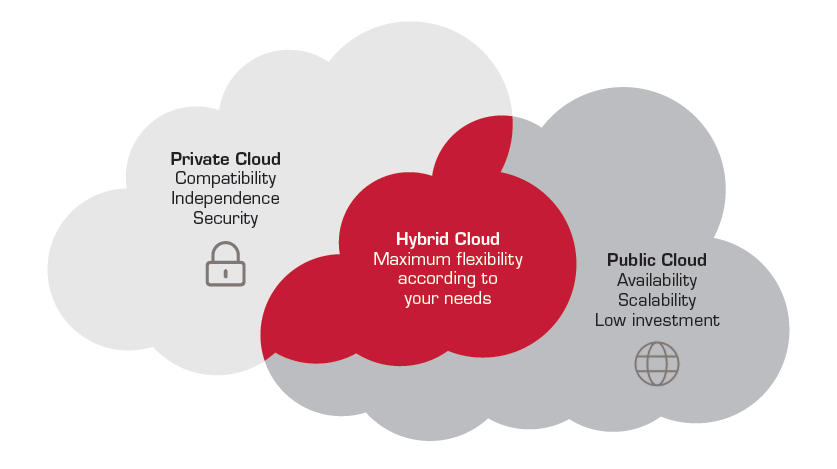
\includegraphics[width=400]{bachproef/img/hybridCloud.png}}
\caption{\textit{Hybrid cloud figuur \autocite{Boris2020hybrid}}}
\label{fig}
\end{figure}
\newpage
\subsection{Service Models}
\label{sec:Service models}

Zoals men eerder schreef wordt cloud computing gevormd door de vijf hiervoor genoemde en beschreven karakteristieken. Verder ook door de vier \textbf{deployment models} waar net over verteld werd en nog drie andere \textbf{service models} waar nu naar gekeken zal worden. deze bestaan namelijk uit:

\begin{itemize}
    \item Software as a Service (SaaS)
    \item Platform as a Service (PaaS)
    \item Infrastructure as a Service (IaaS)
    %\item Network as a Service (NaaS)
\end{itemize}


\subsubsection{SaaS}
\textit{SaaS} is één van de vormen van \textbf{service models} waar de cloud provider applicaties ontwikkelt, onderhoud en deze ter beschikking stelt aan de gebruiker in de vorm van een \textbf{\textit{pay as you go}} model zoals eerder besproken. De cloud provider neemt het hele onderhoudt van de infrastructuur en beveiliging op zich. Via een computer en een internet verbinding kan er gebruik worden gemaakt van de software \autocite{OracleSaaS} \autocite{mell2011nist}.%, een aantal voorbeelden van zulke applicaties zijn bijvoorbeeld:

%\begin{itemize}
%    \item Azure Key Vault \footnote{azure.microsoft.com/nl-nl/services/key-vault}
%    \item AWS Key Management Service \footnote{aws.amazon.com/kms}
%    \item Google Cloud Key Management \footnote{cloud.google.com/security-key-management}
%\end{itemize}

\subsubsection{PaaS}
Bij dit model krijgt de klant de mogelijkheid applicaties te laten lopen op de systemen en ook de keuze om op deze cloud infrastructuur te werken zonder enige zorg aan onderliggende zaken zoals: netwerk, servers, besturing en opslag. Los van deze zaken heeft de gebruiker wel nog altijd autorisatie over de configuraties en beheer van de gelanceerde applicaties en gegevens \autocite{mell2011nist}.

\subsubsection{IaaS}

De mogelijkheid wordt hier voorgesteld bij de gebruiker voor verwerking van data, opslag, netwerken en andere fundamentele computer middelen zodat de gebruiker zelf de keuze heeft om zijn noden te voldoen. De gebruiker beheert de onderliggende cloud infrastructuur niet maar heeft wel controle over de besturing systemen, opslag en gelanceerde applicaties. Verder is er ook de mogelijkheid om de netwerk componenten te configureren voor gelimiteerde toegang \autocite{mell2011nist}.
\newpage
\subsection{Secrets Management als cloud oplossing}
\label{sec:Key managers}
\subsubsection{Azure Key Vault}

Azure Key Vault\footnote{\href{https://azure.microsoft.com/nl-nl/services/key-vault/}{Microsoft Azure Key Vault website}} is een PaaS oplossing dat je toelaat om beveiligd cryptografische sleutels te beheren. Secrets worden onderhouden via deze service. Wanneer bijvoorbeeld, virtuele machines en schijven worden opgezet in de cloud, worden deze door Azure zelf geëncrypteerd. De mogelijkheid is er om zelf een encryptie sleutel te gebruiken om de schijven van virtuele machines te encrypteren. Deze encryptie sleutels kunnen dan via de Azure Key Vault bijgehouden worden. Deze tool laat gecentraliseerd beheer toe voor secrets.

Via het platform kan een secret worden aangemaakt met de kenmerken die eerder werden opgesomd bij het \textit{application-pull} model:

\begin{itemize}
    \item Central management
    \item Access policies
    \item Auditing
    \item Ephemeral credentials
    \item Compartmentalization
    \item Facilitates rotation
\end{itemize}

De secret wordt centraal beheerd via een vault dat kan worden aangemaakt via het Azure platform. Via \textit{Identity Access Management (IAM)} kan er beheerd worden waar een gebruiker toegang tot heeft en welke acties deze gebruiker heeft uitgevoerd \autocite{ganatra2019}. Dit wordt verder ondersteund door het activiteitenlogboek dat Azure aanbiedt binnen de key vault service. Als secrets worden aangemaakt wordt er de keuze gegeven of er een activatie of expiratie moment wordt opgegeven. Dit zorgt er voor dat gegevens vluchtig kunnen zijn. Men kan meerdere vaults maken met meerdere gegevens die voor allerlei applicaties gebruikt worden. Deze worden geleverd aan applicaties via service principals. Dit zijn applicaties dat binnen Azure Active Directory worden aangemaakt om toegang te verkrijgen tot resources in Azure. Deze kunnen gebruikt worden om secrets op te halen voor applicaties. Secrets zijn nooit hard coded en kunnen binnen de key vault opnieuw gegenereerd worden. Deze worden bijgewerkt en applicaties verkrijgen zo geautomatiseerd hun bijgewerkte sleutel. Er zijn meerdere manieren om sleutel generatie en rotatie te automatiseren na een bepaald tijdsinterval. De meest gebruikte manier is via Azure Automation met een geautomatiseerd script \autocite{Majumder2019} \autocite{Marczak2020}.

%Je verwijst bij elke bewering die je doet, vakterm die je introduceert, enz. naar je bronnen. In \LaTeX{} kan dat met het commando \texttt{$\backslash${textcite\{\}}} of \texttt{$\backslash${autocite\{\}}}. Als argument van het commando geef je de ``sleutel'' van een ``record'' in een bibliografische databank in het Bib\LaTeX{}-formaat (een tekstbestand). Als je expliciet naar de auteur verwijst in de zin, gebruik je \texttt{$\backslash${}textcite\{\}}. Soms wil je de auteur niet expliciet vernoemen, dan gebruik je \texttt{$\backslash${}autocite\{\}}. In de volgende paragraaf een voorbeeld van elk.